\subsubsubsubsection{Direction}
\begin{figure}[h]
\centering
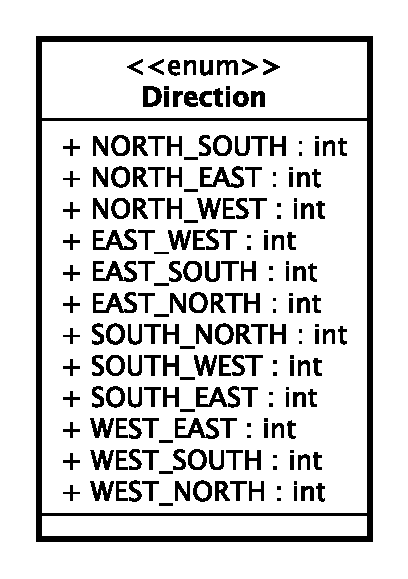
\includegraphics[scale=0.6,keepaspectratio]{images/solution/app/backend/direction.eps}
\caption{\pReactiveComponent::Direction}
\label{fig:sd-app-direction}
\end{figure}
\FloatBarrier
\begin{itemize}
  \item \textbf{\descr} \\
    It represents the direction that a moving entity has while treading a
    street or a crossroads.
  \item \textbf{\values}
  \begin{itemize}
    \item[+] \texttt{NORTH\_SOUTH: int} \\
    Straight direction, from north to south.
    \item[+] \texttt{NORTH\_EAST: int} \\
    Turning left direction, from north to east.
    \item[+] \texttt{NORTH\_WEST: int} \\
    Turning right direction, from north to west.
    \item[+] \texttt{EAST\_WEST: int} \\
    Straight direction, from east to west.
    \item[+] \texttt{EAST\_SOUTH: int} \\
    Turning left direction, from east to south.
    \item[+] \texttt{EAST\_NORTH: int} \\
    Turning right direction, from east to north.
    \item[+] \texttt{SOUTH\_NORTH: int} \\
    Straight direction, from south to north.
    \item[+] \texttt{SOUTH\_WEST: int} \\
    Turning left direction, from south to west.
    \item[+] \texttt{SOUTH\_EAST: int} \\
    Turning right direction, from north to east.
    \item[+] \texttt{WEST\_EAST: int} \\
    Straight direction, from west to east.
    \item[+] \texttt{WEST\_SOUTH: int} \\
    Turning left direction, from west to south.
    \item[+] \texttt{WEST\_NORTH: int} \\
    Turning right direction, from west to north.
  \end{itemize}
\end{itemize}